\documentclass[../sparc.tex]{subfiles}
\graphicspath{{\subfix{../images/}}}
\begin{document}

%%%%%%%%%%%%%%%%%%%%%%%%%%%%%%%%%%%%%%%%%%%%%%%%%%%%%%%%%%%%%%%%%%%%%%%%%%%%%%%%
\newpage
\section{Теория ритма}
\index{Музыка!Ритм}

Наш путь в музыку начнётся с разбора теории построения \emph{ритмов}.
Большинство из нас представляют, что такое ритм -- у многих именно он вызывает
например рефлекс покачивания головой в такт, или машинальное отстукивание ритма
на столешнице стола, когда думаем над чем-то.

Чтобы понять, как строится ритм, необходимо знать две простые вещи, о которых мы
сейчас поговорим.

%%%%%%%%%%%%%%%%%%%%%%%%%%%%%%%%%%%%%%%%%%%%%%%%%%%%%%%%%%%%%%%%%%%%%%%%%%%%%%%%
\subsection{Понятие \emph{такта}}
\index{Музыка!Ритм!Такт}

Во-первых, музыкальное произведение делится на отрезки времени, называемые
\emph{тактами} -- как правило одинаковой длительности.\footnote{Музыка отличается
большим разнообразием, и композиторы придумывают всё новые трюки, как получить
желаемое впечатление у слушателя, поэтому здесь мы говорим с некоторыми
допущениями.}

На рисунке ниже показано, как может выглядеть музыкальная композиция из шести
тактов:

\begin{tikzpicture}
  \draw[thick, ->] (0, 0.5) -- (12, 0.5) node[anchor=north west] {t};
  \foreach \x/\n in {0/1, 2/2, 4/3, 6/4, 8/5, 10/6} {
    \draw (\x, 0) -- (\x, 1) -- (\x, 1) node[midway, above] {\n};
  };
\end{tikzpicture}

Протяжённость одного такта во времени определяется быстротой ритма, и про это мы
поговорим позже. Пока можно представить, что один отрезок занимает одну условную
единицу времени. Можете принять эту условую единицу за отрезок времени, удобный
для вашего восприятия -- например, одну секунду.

Во-вторых, эти такты делятся на ещё более мелкие части, по которым, как по
``ячейкам'', раскладываются различные звуки. Достаточно большая часть музыки
пронизана математикой, и первое математическое, с чем мы столкнёмся -- это
простые дроби. Одним из популярных способов деления такта на части является
$\frac{4}{4}$ или, по-другому называемый ``четыре четверти''. В таком способе
деления такта в него умещается ровно единица некоторого условного времени, про
которое мы говорили выше.\footnote{Существуют более сложные способы деления
такта на части, которые дают суммарное значение меньше или больше единицы -- про
это мы поговорим позднее.}

Если мы поделим каждый такт на четыре части, то получим следующую картину:

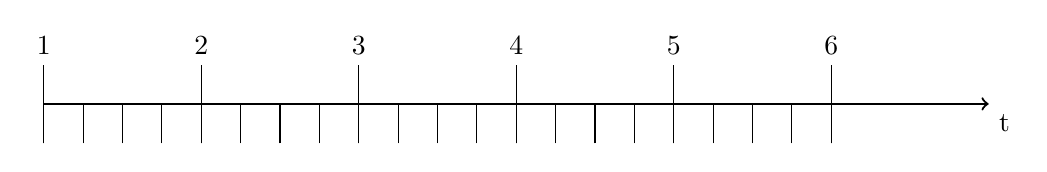
\begin{tikzpicture}
  \draw[thick, ->] (0, 0.5) -- (12, 0.5) node[anchor=north west] {t};
  \foreach \x/\n in {0/1, 2/2, 4/3, 6/4, 8/5, 10/6} {
    \draw (\x, 0) -- (\x, 1) -- (\x, 1) node[midway, above] {\n};
  };

  \foreach \x/\n in {0, 0.5, ..., 10} {
    \draw (\x, 0) -- (\x, 0.5);
  };
\end{tikzpicture}

Возьмём отдельный такт и посмотрим на него внимательно:

\begin{tikzpicture}
  \draw[thick] (0, 0.5) -- (8, 0.5) node[anchor=north west] {t};
  \foreach \x/\n in {0/1, 8/2} {
    \draw (\x, 0) -- (\x, 1)  -- (\x, 1) node[midway, above] {\n};
  };

  \foreach \x in {0, 2, ..., 6} {
    \draw (\x, 0) -- (\x, 0.5) node[pos=0.25, right] {$ \frac{1}{4} $};
  };
\end{tikzpicture}

Если просуммируем все части, то снова получим единицу:

\begin{equation}
  \frac{1}{4} + \frac{1}{4} + \frac{1}{4} + \frac{1}{4} = \frac{1}{1}
\end{equation}

На каждую из четвертей можно задать какой-то звук -- пока нам не важно, насколько
он будет музыкальный. Допустим, что три четверти будут звучать с частотой 50Гц,
и одна часть -- с частотой 100Гц:

\begin{tikzpicture}
  \draw[thick] (0, 0.5) -- (8, 0.5) node[anchor=north west] {t};
  \foreach \x/\n in {0/1, 8/2} {
    \draw (\x, 0) -- (\x, 1) -- (\x, 1) node[midway, above] {\n};
  };

  \foreach \x in {0, 2, ..., 6} {
    \draw (\x, 0) -- (\x, 0.5) node[pos=0.25, right] {$ \frac{1}{4} $};
  };

  \foreach \x/\freq in {0/50, 2/50, 4/50, 6/100} {
    \draw (\x, 0) -- (\x, 0.5) node[pos=1.5, right] {\freq Гц};
  };
\end{tikzpicture}

Поздравляю -- мы только что получили простой ритм. Попробуем запрограммировать
его, беря за длину такта \texttt{T} одну секунду, или 1000000 (миллион)
микросекунд.

Между ``ударами'' необходимо поставить короткую задержку (например, в 100 мс),
чтобы удары одинаковой частоты, идущие один за другим, не сливались в один
долгий звук.

\begin{minted}{cpp}
// Номер порта, куда подключен динамик.
const int SPEAKER = 2;

void setup() {
  pinMode(SPEAKER, OUTPUT);
}

// Функция воспроизведения звука указанной частоты.
void play_tone(int port, float f, long t) {
  const int T = 1000000 / f;
  int d = T / 2;
  int count = t / T;
  for (int i = 0; i < count; i++) {
    digitalWrite(port, HIGH);
    delayMicroseconds(d);
    digitalWrite(port, LOW);
    delayMicroseconds(d);
  }
}

void loop() {
  const long T = 1000000; // Длина такта в микросекундах
  play_tone(SPEAKER, 50,  T / 4); // Четверть
  delay(100); // Задержка между звуками
  play_tone(SPEAKER, 50,  T / 4); // Четверть
  delay(100);
  play_tone(SPEAKER, 50,  T / 4); // Четверть
  delay(100);
  play_tone(SPEAKER, 100, T / 4); // Четверть
  delay(100);
}
\end{minted}

Можно теперь взять что-то посложнее.

%%%%%%%%%%%%%%%%%%%%%%%%%%%%%%%%%%%%%%%%%%%%%%%%%%%%%%%%%%%%%%%%%%%%%%%%%%%%%%%%
\subsection{Более сложные ритмы}

Возможно некоторые из вас знают такую зажигательную композицию, как ``We Will
Rock You'' в исполнении группы Queen\footnote{Официальное музыкальное видео на
данную композицию можно посмотреть здесь:
\url{https://www.youtube.com/watch?v=-tJYN-eG1zk}}. Данная композиция имеет
чётко выраженный, легко узнаваемый ритм, который можно упрощенно описать как
``два притопа, один прихлоп'', вокруг которого строится вся композиция -- вы сами
можете достаточно легко повторить этот ритм, коротко топая ногой два раза, и
потом делая ``долгий'' хлопок руками.

\begin{figure}[ht]
  \centering
  \begin{tikzpicture}
    \draw[thick] (0, 0.5) -- (8, 0.5) node[anchor=north west] {t};
    \foreach \x/\n in {0/1, 8/2} {
      \draw (\x, 0) -- (\x, 1) -- (\x, 1) node[midway, above] {\n};
    };

    \foreach \x in {0, 2} {
      \draw (\x, 0) -- (\x, 0.5) node[pos=0.25, right] {$ \frac{1}{4} $};
    };

    \draw (4, 0) -- (4, 0.5) node[pos=0.25, right] {$ \frac{1}{2} $};

    \foreach \x/\freq in {0/50, 2/50} {
      \draw (\x, 0) -- (\x, 0.5) node[pos=1.5, right] {\freq Гц};
    };
    \draw (4, 0) -- (4, 0.5) node[pos=1.5, right] {100 Гц};
  \end{tikzpicture}
  \caption{Ритм мелодии ``We Will Rock You'' группы Queen (упрощенная версия.)}
  \label{fig:queen-we-will-rock-you-rhythm-1}
\end{figure}

Структура этого ритма может быть описана следующим набором простых дробей
(\ref{fig:queen-we-will-rock-you-rhythm-1}.) Частоты звуков мы, опять же, берём
произвольно.

Как мы видим из рисунка \ref{fig:queen-we-will-rock-you-rhythm-1}, деление такта
на части не обязательно должно быть всегда равномерным -- здесь мы получили две
четверти и одну половину.  Для сложения простых дробей нам необходимо их
привести к общему знаменателю.  Таким образом, в сумме у нас опять выходит
единица (см. формулу \ref{equation:queen-we-will-rock-you-rhythm-1}.)

\begin{equation}
  \frac{1}{4} + \frac{1}{4} + \frac{1}{2} = \frac{1}{4} + \frac{1}{4} + \frac{2}{4} = \frac{4}{4} = \frac{1}{1} = 1
  \label{equation:queen-we-will-rock-you-rhythm-1}
\end{equation}

%%%%%%%%%%%%%%%%%%%%%%%%%%%%%%%%%%%%%%%%%%%%%%%%%%%%%%%%%%%%%%%%%%%%%%%%%%%%%%%%
\subsection{Музыкальная запись ритма}

С точки зрения музыкальной нотации, данный ритм можно записать примерно
следующим образом (см. рисунок \ref{fig:lilypond-queen-1}.)

\begin{figure}[ht]
  \centering
  \begin{lilypond}
    \relative c' {
      \numericTimeSignature
      \time 4/4
      e,4 e4 e'2
    }
  \end{lilypond}
  \caption{Ритм мелодии ``We Will Rock You'' в музыкальной нотации (упрощенная версия.)}
  \label{fig:lilypond-queen-1}
\end{figure}

Если вы не знакомы с музыкальной нотацией (т.е. способом записи музыки), и
изображение выглядит для вас совершенно непонятно, то не отчаивайтесь -- на
данном этапе нам достаточно увидеть, что есть три ``закорючки'', которые
обозначают звуки разной длительности: ``\quarterNote'' ($\frac{1}{4}$),
``\quarterNote'' ($\frac{1}{4}$) и ``\halfNote'' ($\frac{1}{2}$).

Расположение ``закорючек'' слева на право говорит нам о порядке ``извлечения''
звуков из музыкальных инструментов, а каждый вид начертания ``закорючки''
соответствует длительности звука, согласно следующей таблице
(\ref{table:music-notes-legths}.)

\begin{table}[ht]
\centering
\def\arraystretch{2.5}%
\begin{tabular}{|m{3cm}|m{4cm}|m{3.5cm}|}
  \hline
  \textbf{Начертание} & \textbf{Длительность} & \textbf{Название} \\
  \hline
  {\Large \wholeNote} & {\Large $\frac{1}{1}$} & Целая \\[2ex]
  \hline
  {\Large \halfNote}      & {\Large $\frac{1}{2}$}  & Половина \\[2ex]
  \hline
  {\Large \quarterNote}   & {\Large $\frac{1}{4}$}  & Четверть \\[2ex]
  \hline
  {\Large \eighthNote}    & {\Large $\frac{1}{8}$}  & Восьмая \\[2ex]
  \hline
  {\Large \sixteenthNote} & {\Large $\frac{1}{16}$} & Шестнадцатая \\[2ex]
  \hline
\end{tabular}
\caption{Некоторые возможные длительности нот.}
\label{table:music-notes-legths}
\end{table}

Существуют и более длинные и более короткие ноты, но они встречаются реже, чем
перечисленные в таблице \ref{table:music-notes-legths}, поэтому для краткости мы
их рассматривать не будем.

Какие выводы мы можем сделать в итоге? Что в музыкальной нотации звуки, которые
необходимо ``извлечь'' из музыкального инструмента, записываются слева на право,
как и обычный, привычный нам русский текст (или английский, к слову говоря.)

Мы можем расположить музыкальную запись для удобства нашего понимания на
графике, где ось $\mbox{X}$ будет обозначать время, идущее слева направо:

\begin{figure}[ht]
  \centering
  \begin{lilypond}
    \relative c' {
      \numericTimeSignature
      \time 4/4
      e,4 e4 e'2
    }
  \end{lilypond}
  \begin{tikzpicture}
    \draw[thick, ->] (0, 0.5) -- (12, 0.5) node[anchor=north east] {Время};
  \end{tikzpicture}

  \caption{Музыкальный ``график''.}
  \label{fig:lilypond-queen-1}
\end{figure}

С точки зрения программирования, код воспроизведения ритма может быть следующим:

\begin{minted}{cpp}
// Здесь пропущен уже известный вам код настройки системы и реализации
// функции воспроизведения звука.

void loop() {
  const long T = 1000000; // Длина такта в микросекундах
  play_tone(SPEAKER, 50, T / 4); // Четверть
  delay(100);
  play_tone(SPEAKER, 50, T / 4); // Четверть
  delay(100);
  play_tone(SPEAKER, 100, T / 2); // Половина
  delay(100);
}
\end{minted}

Теперь нам нужно более точно определить, какова длительность целого отрезка
времени, чтобы посчитать длину его частей.

%%%%%%%%%%%%%%%%%%%%%%%%%%%%%%%%%%%%%%%%%%%%%%%%%%%%%%%%%%%%%%%%%%%%%%%%%%%%%%%%
\subsection{Темп музыки}
\index{Музыка!Ритм!Удары в минуту (Beats Per Minute, BPM)}
\newglossaryentry{BPM}{name=BPM, description={Beats Per Minute -- удары в минуту}}

\emph{Темпом} в музыке называется скорость исполнения музыки, если говорить
упрощенно. В современной музыке темп измеряется в \emph{ударах в минуту}
(буквальный перевод английского ``Beats per Minute'', сокращённо называемый
\emph{\gls{BPM}}.)

Темп в музыке может задаваться с помощью специального маятника, который
раскачивается из стороны в сторону с равномерной скоростью, делая удары (или
щелчки) в крайних положениях. Такой маятник называется \emph{метрономом}.

\begin{figure}[h]
  \centering
  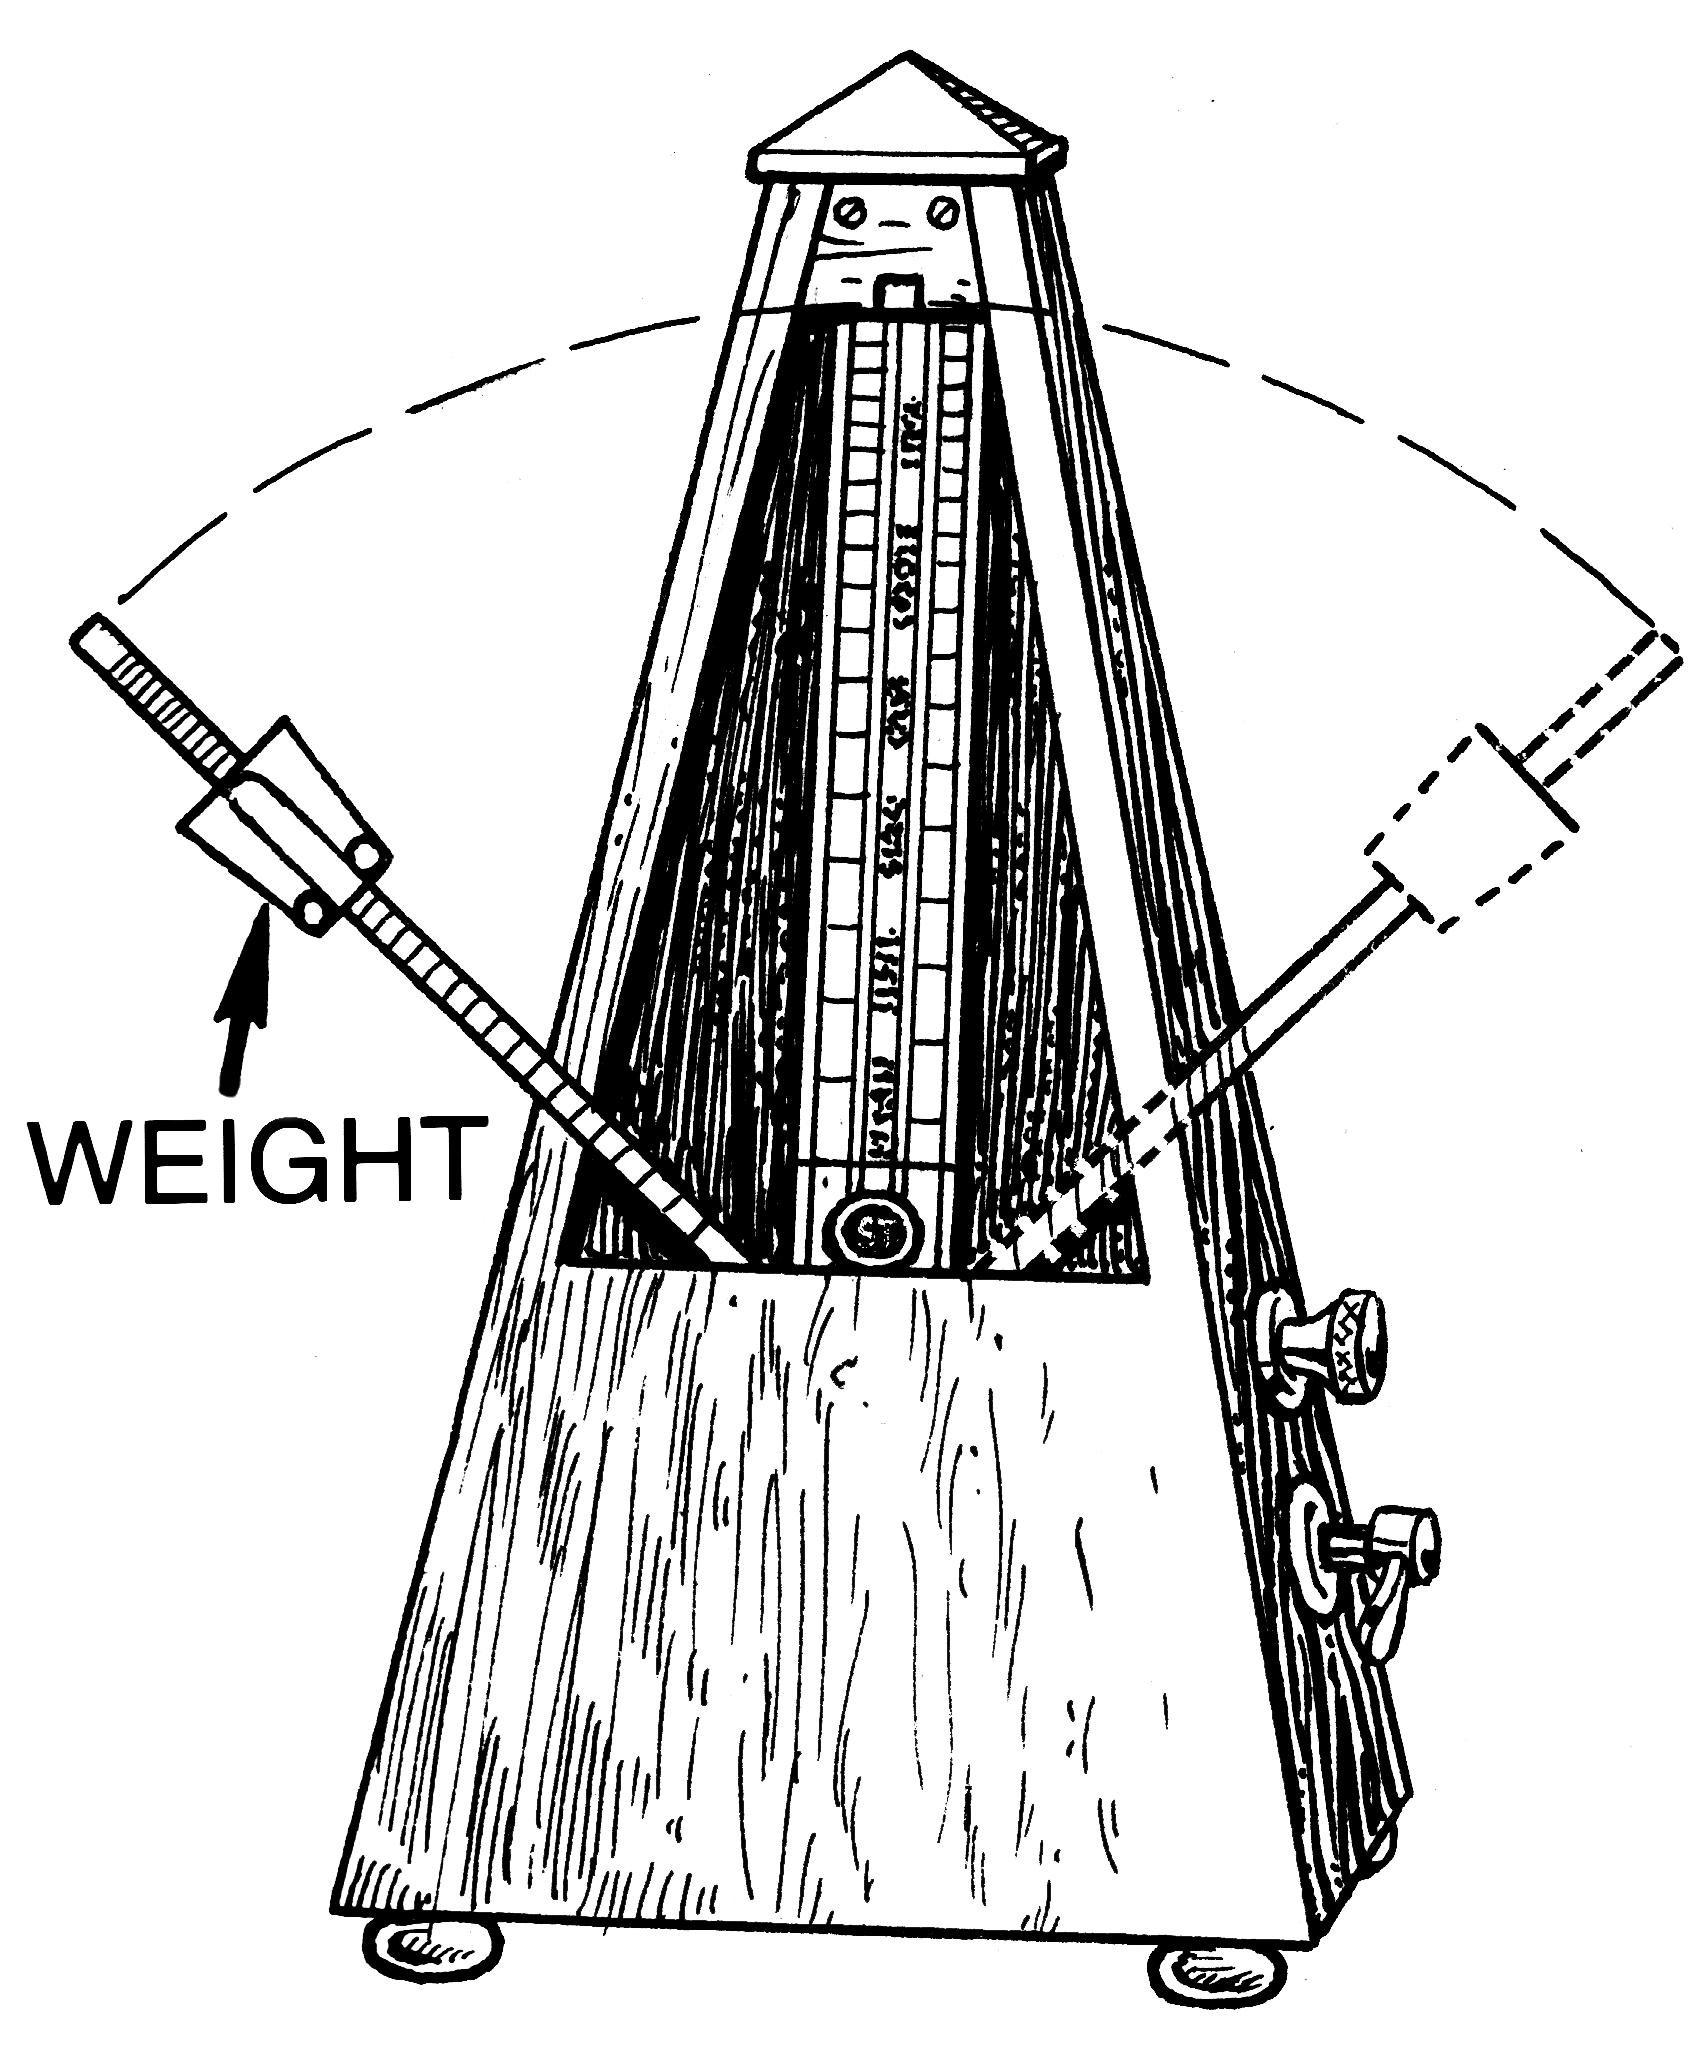
\includegraphics[width=10cm]{Metronome}
  \caption{Схематическое изображение механического метронома (источник:
    \url{https://commons.wikimedia.org/wiki/File:Metronome_(PSF).png}).}
  \label{fig:sound-metronome}
\end{figure}

В современном мире роль механического маятника часто заменяет специальное
компактное электронное устройство или даже приложение для мобильного телефона,
издающее щелчки через равные промежутки времени с заданной скоростью.

Чем больше ударов в минуту, тем выше темп -- и выше скорость ритма. Примерами BPM
могут служить 60, 80 и 100 ударов в минуту.

Но как связать скорость ритма с делением такта на части? Оказывается,
равномерные удары метронома задают длину одной четверти ($\frac{1}{4}$), на
которые у нас в примерах выше делился такт.

Таким образом, если темп ритма задан в 100 ударов в минуту, то это значит, что в
минуту помещается ровно 100 четвертей.

\begin{tikzpicture}
  \draw[thick] (0, 0.5) -- (10, 0.5) node[anchor=north west] {t};
  \draw (0, -0.5) -- (0, 1.5);
  \draw (10, -0.5) -- (10, 1.5);
  \draw (1, 1.5) node[anchor=north west] {1 минута (60 секунд) / 100 ударов};
  \foreach \x in {0.0, 0.1, 0.2, ..., 10.0} {
    \draw (\x, 0) -- (\x, 1);
  };
\end{tikzpicture}

Расстояние между двумя ударами можно рассчитать по формуле \ref{equation:bpm}.

\begin{equation}
  \frac{\mbox{60 с}}{\mbox{100 ударов}} = \mbox{0.6 с} = \mbox{60 мс} = \mbox{60000 мкс}
  \label{equation:bpm}
\end{equation}

Исходя из формулы \ref{equation:bpm} мы получаем длительность одной четверти в
0.6с. Но для удобства расчётов мы должны посчитать длину целого такта, а не его
части. Поскольку в такт, который мы рассматриваем в примере, помещается четыре
четверти, для нахождения целого достаточно умножить четверть на четыре (см.
формулу \ref{equation:whole-note-calcualtion-1}).

\begin{equation}
  \frac{1}{4} * 4 = \frac{4}{4} = \frac{1}{1} = 1
  \label{equation:whole-note-calcualtion-1}
\end{equation}

Зная это, можно вывести общую формулу \ref{equation:whole-note-calcualtion-2}
для вычисления длительности целого такта.

\begin{equation}
  \frac{\mbox{60 c}}{\mbox{BPM}} * 4 = \mbox{Длина целого такта}
  \label{equation:whole-note-calcualtion-2}
\end{equation}

Теперь мы можем музыкально точно рассчитать длину звуков, из которых строится
ритм произведения -- в том числе, композиции ``We Will Rock You'', которую мы
рассматривали выше. Для неё BPM равен примерно 80 ударов в минуту.\footnote{В
разных источниках могут быть указаны разные варианты BPM, но в целом темп этой
композиции обычно находится в диапазоне от 84 до 88 ударов в минуту.}

Попробуем запрограммировать его.

\begin{minted}{cpp}
// Номер порта, куда подключен динамик.
const int SPEAKER = 2;

void setup() {
  pinMode(SPEAKER, OUTPUT);
}

// Функция воспроизведения звука указанной частоты.
void play_tone(int port, float f, long t) {
  const int T = 1000000 / f;
  int d = T / 2;
  int count = t / T;
  for (int i = 0; i < count; i++) {
    digitalWrite(port, HIGH);
    delayMicroseconds(d);
    digitalWrite(port, LOW);
    delayMicroseconds(d);
  }
}

void loop() {
  const int BPM = 80; // Удары в минуту

  // Одна минута в микросекундах
  const long MINUTE = 60000000;

  // Длина целого такта в микросекундах
  const long T = (MINUTE / BPM) * 4;

  play_tone(SPEAKER, 50, T / 4); // Четверть
  delay(100);
  play_tone(SPEAKER, 50, T / 4); // Четверть
  delay(100);
  play_tone(SPEAKER, 100, T / 2); // Половина
  delay(100);
}
\end{minted}

Если вы загрузите данный проект в Arduino, то обнаружите, что ритм получился
слишком медленный и не совпадает с темпом оригинальной композиции. Так произошло
потому, что мы не учли один важный момент -- в такте должно быть две группы ``два
притопа, один прихлоп'' (см. рисунок \ref{fig:lilypond-queen-2}.)

\begin{figure}[ht]
  \centering
  \begin{lilypond}
    \relative c' {
      \numericTimeSignature
      \time 4/4
      e,8 e8 e'4 e,8 e8 e'4
    }
  \end{lilypond}
  \caption{Ритм мелодии ``We Will Rock You'' в музыкальной нотации (полная версия.)}
  \label{fig:lilypond-queen-2}
\end{figure}

Из-за этого в оригинале композиция кажется в два раза быстрее -- не потому, что
там выше BPM, а из-за того, что сами ноты короче.

Адаптируем наш код соответствующим образом.

\begin{minted}{cpp}
// ...

void loop() {
  const int BPM = 80; // Удары в минуту

  // Одна минута в микросекундах
  const long MINUTE = 60000000;

  // Длина целого такта в микросекундах
  const long T = (MINUTE / BPM) * 4;

  play_tone(SPEAKER, 50, T / 8); // Восьмая
  delay(100);
  play_tone(SPEAKER, 50, T / 8); // Восьмая
  delay(100);
  play_tone(SPEAKER, 100, T / 4); // Четверть
  delay(100);
  play_tone(SPEAKER, 50, T / 8); // Восьмая
  delay(100);
  play_tone(SPEAKER, 50, T / 8); // Восьмая
  delay(100);
  play_tone(SPEAKER, 100, T / 4); // Четверть
  delay(100);
}
\end{minted}

Ритм готов, однако мы всё ещё выбираем частоты наших ``инструментов''
произвольно -- пришло время это исправить.

\end{document}
